\section{Results}

The latency and energy improvements of inference and online training with our engine for 8 different benchmarks are shown in Figures~\ref{inference_results} and~\ref{training_results},  respectively. We considered the best case of mobile-only and cloud-only as our baseline. JointDNN can achieve up to 66\% and 86\% improvements in latency and energy consumption, respectively during inference. Communication cost increases linearly with batch size while this is not the case for computation cost and it grows with much lower rate, as depicted in~\ref{weights_changed}(b). Therefore, a key observation is that as we increase the batch size, the mobile-only approach becomes more preferable. 


\begin{figure}[b]
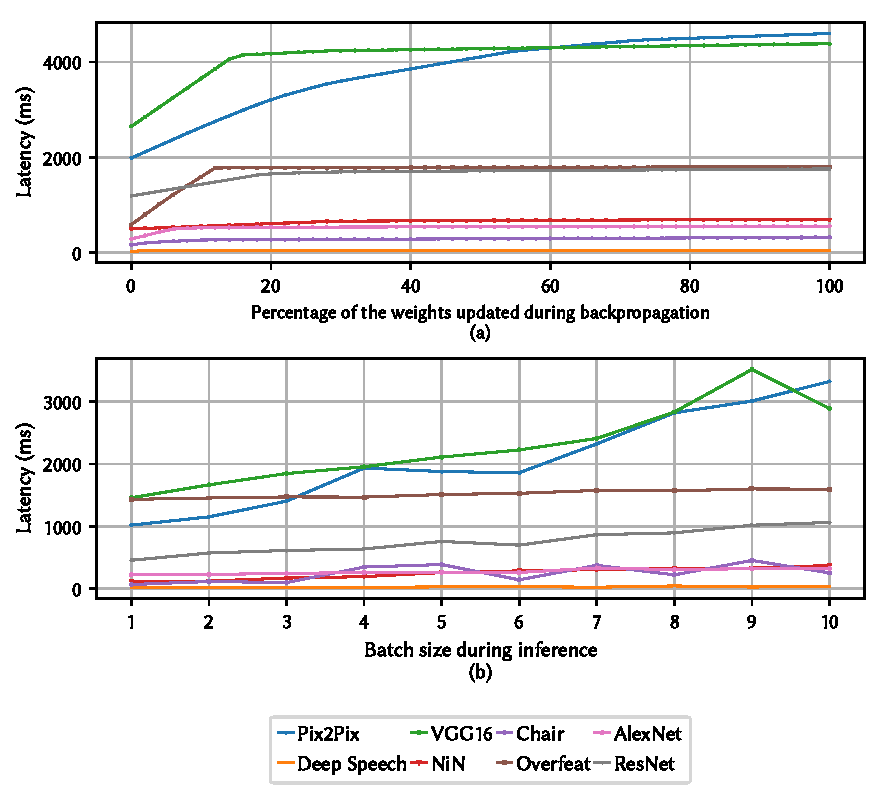
\includegraphics[width=\linewidth]{training_weights_results}
\caption{(a)~Latency of one epoch of online training using JointDNN algorithm vs percentage of updated weights (b)~Latency of mobile-only inference vs. batch size.}\label{weights_changed}
\end{figure}

During online training, the huge communication overhead of transmitting the updated weights will be added to the total cost. Therefore, in order to avoid downloading this large data, only a few back-propagation steps are computed in the cloud server. We performed a simulation by varying the percentage of updated weight. As the percentage of updated weights increases, the latency and energy consumption becomes constant which is shown in~Figure~\ref{weights_changed}. This is the  result of the fact that all the back-propagations will be performed on the mobile device and weights are not transfered from the cloud to the mobile. JointDNN can achieve improvements up to 73\% in latency and 56\% in energy consumption during inference.

\begin{figure}[t]
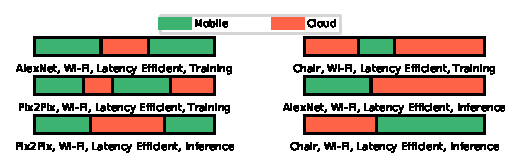
\includegraphics{interesting_patterns}
\caption{Interesting schedules of execution for three types of DNN architectures.} \label{interesting_patterns}
\end{figure}

Different patterns of scheduling are demonstrated in Figure~\ref{interesting_patterns}. They represent the optimal solution in Wi-Fi network while optimizing for latency. They show how the computations in DNN is divided between the mobile and the cloud. As it can be seen, discriminative models (e.g. AlexNet), inference follows a mobile-cloud pattern and training follows a mobile-cloud-mobile pattern. The intuition is that the last layers are computationally intensive \textit{(fc)} with small data sizes, which require a low communication cost, therefore, last layers tend to be computed on the cloud. For generative models (e.g. Chair), the execution schedule of inference is the opposite of discriminative networks, in which the last layers are generally huge and in the optimal solution they are computed on the mobile. Lastly, for autoencoders, where both the input and output data sizes are large, the first and last layers are computed on the mobile.

% \begin{figure}
% 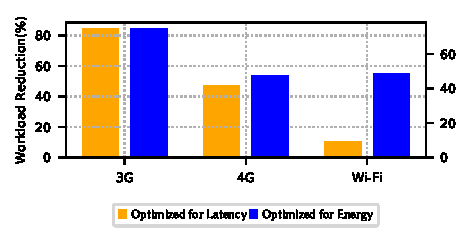
\includegraphics{cloud_improvement}
% \caption{Workload reduction of the cloud server in different mobile networks} \label{cloud_improvement}
% \end{figure}

JointDNN pushes some parts of the computations toward the mobile device. As a result this will lead to less workload on the cloud server. As we see in Table~\ref{cloud_improvement}, we can reduce the cloud server's workload up to 84\% and 53\% on average, which enables the cloud provider to service more users, while obtaining higher performance and lower energy consumptions compared to single-platform approaches.  

\begin{table}[h]
\centering
\caption{Workload reduction of the cloud server in different mobile networks}
\label{cloud_improvement}
\begin{tabular}{|c|c|c|c|}
\hline
\textbf{Optimization Target} & \textbf{3G (\%)} & \textbf{4G (\%)} & \textbf{Wi-Fi (\%)} \\ \hline
Latency                      & 84               & 49               & 12                  \\ \hline
Energy                       & 73               & 49               & 51                  \\ \hline
\end{tabular}
\end{table}

\subsection{Communication Dominance}
Execution time and energy breakdown for AlexNet, which is noted as a representative for the state-of-the-art architectures deployed in cloud servers, is depicted in Figure~\ref{alexnet_extracted}. The cloud-only approach is dominated by the communication costs. As demonstrated in Figure~\ref{alexnet_extracted}, 99\%, 93\% and 81\% of the total execution time is used for communication in case of 3G, 4G, and Wi-Fi, respectively. This relative portion also applies to energy consumption. Comparing the latency and energy of the communication to those of mobile-only approach, we notice that mobile-only approach for AlexNet is better than the cloud-only approach in all the mobile networks. We apply lossless compression methods in order to reduce the effect of the communication, which will be covered in the next section. 

\begin{figure}[t]
\centering
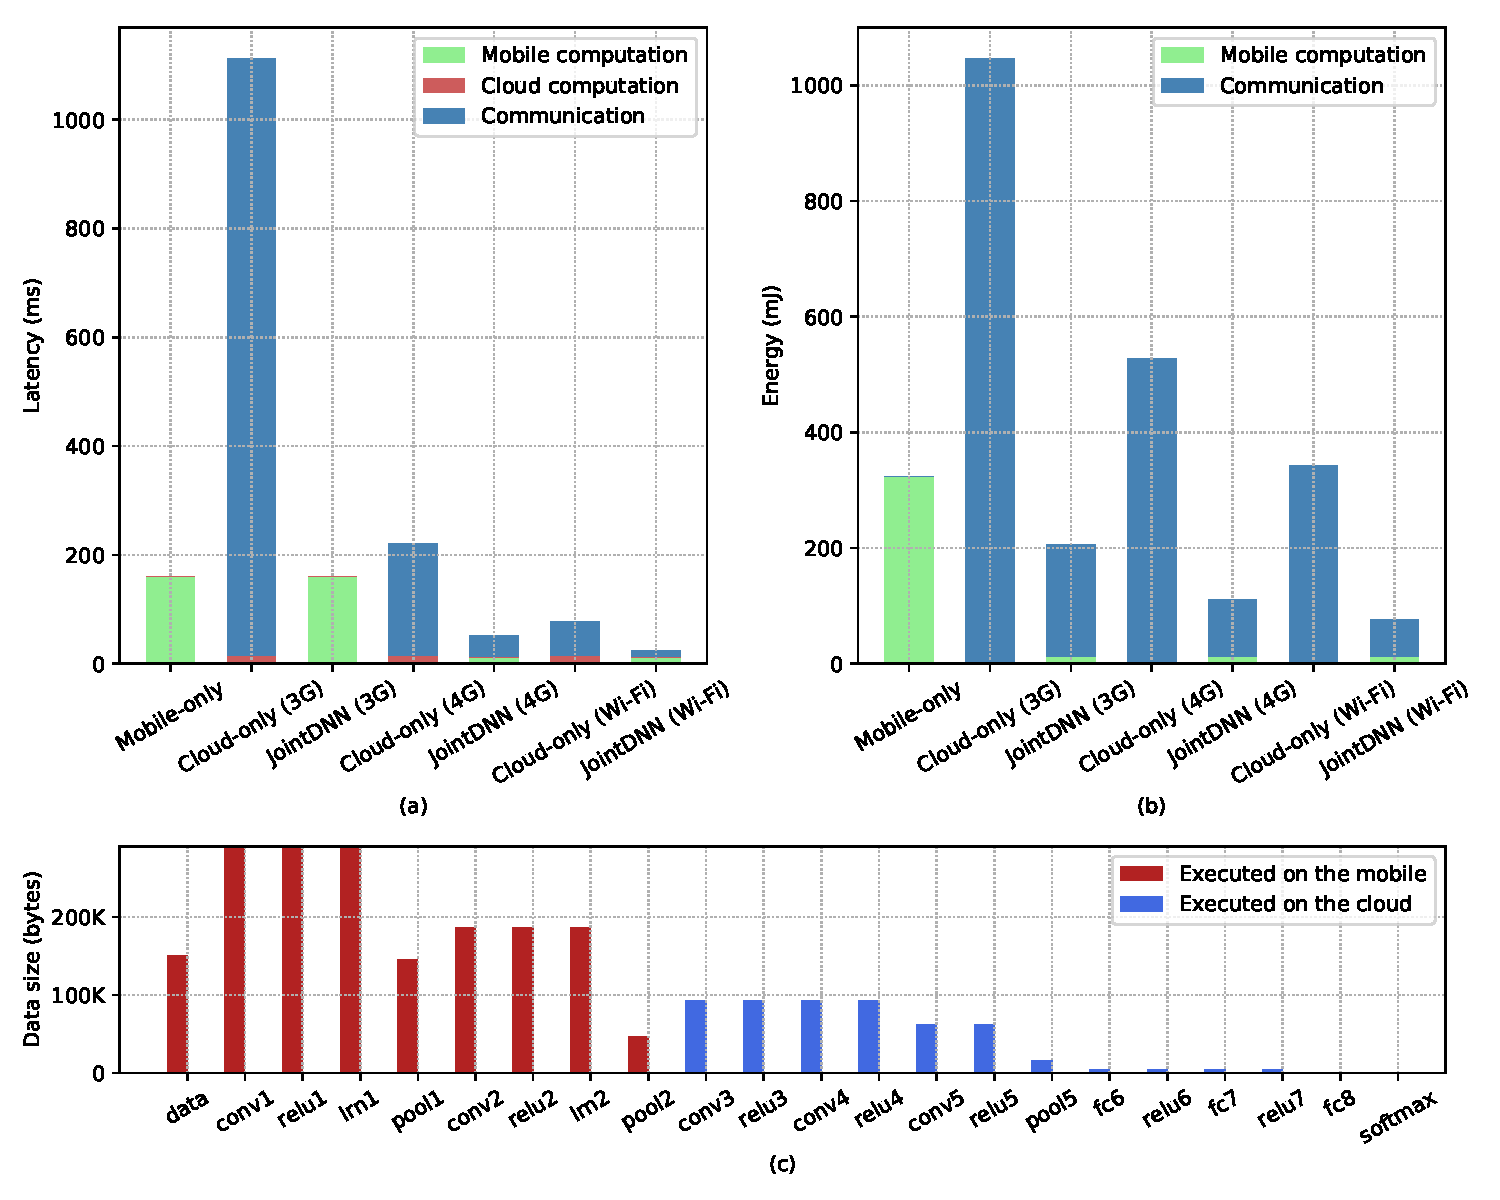
\includegraphics[width=\linewidth]{alexnet_extracted}
\caption{(a) Execution time of AlexNet optimized for performance (b) Mobile energy consumption of AlexNet optimized for energy (c) Data size of the layers in AlexNet and the scheduled computation, where the first nine layers are computed on the mobile and the rest on the cloud, which is the optimal solution w.r.t. both performance and energy.}
\label{alexnet_extracted}
\end{figure}


\subsection{Layer Compression}

The preliminary results of our experiments show that more than $75\%$ of the total energy and delay cost in DNNs are caused by communication in the collaborative approach. This cost is directly proportional to the size of the layer being downloaded to or uploaded from the mobile device. Because of the complex feature extraction process of DNNs, the size of some of the intermediate layers are even larger than network's input data. For example, this ratio can go as high as $10\times$ in VGG16. To address this bottleneck, we investigated compression of the data before any communication. This process can be applied to different DNN architecture types; however, we only considered CNNs due to their specific characteristics explained later in details. 

\begin{figure}[b]
\centering
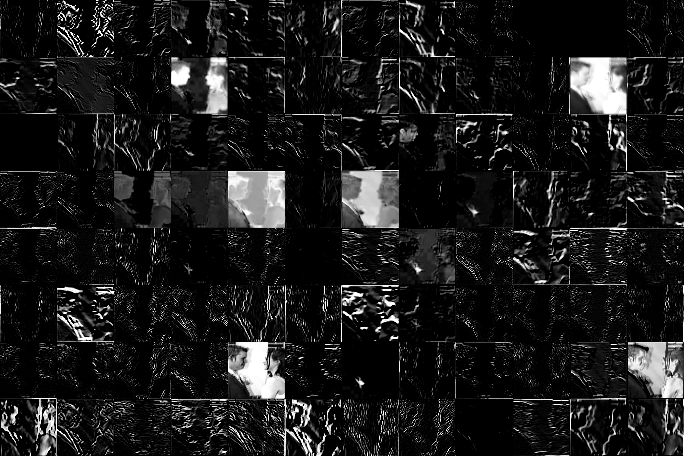
\includegraphics[width=\linewidth]{picCNN}
\caption{Layer output after passing the input image through \textit{conv}, \textit{relu} and \textit{lrn}. Channels are preserving the general structure of the input image and large ratio of the output data is black (zero) due to existence of \textit{relu}. Tiling is used to put all 96 channels together.}
\label{fig:picCNN}
\end{figure}

CNN architectures are mostly used for image and video recognition applications. Because of the spatially local preservation characteristics of \textit{conv} layers, we can assume that the output of the first convolution layers are following the same structure as the input image, as shown in Figure~\ref{fig:picCNN}. Moreover, a big ratio of layer outputs are expected to be zero due to the presence of the relu layer. Our observations shows that the ratio of neurons equal to zero \textit{(ZR)} varies from 50\% to 90\% after \textit{relu} in CNNs. These two characteristics, layers being similar to the input image, and large proportion of their data being a single value, suggest that we can employ existing image compression techniques to their output. 


% This can be ignored! Specially if we don't want to bring that one PNG and JPEG sentence! 
There are two general categories of compression techniques, lossy and lossless~\cite{InformationTheoryCover}. In lossless techniques it is possible to reconstruct the original information completely. On the contrary, lossless techniques use approximations and the original data cannot be reconstructed. In our experiments, we examined the impact of compression using PNG, a lossless technique, based on encoding of frequent sequences in an image. 

% Quantization %% UP TO HERE!
Even though the data type of DNN parameters in typical implementations are 32-bits floating-points, most image formats are based on 3-bytes RGB color triples. Therefore, to compress the layer in the same way as 2D pictures, the floating-point data should be quantized into 8-bits fixed-point. Recent studies show representing the parameters of DNNs with only 4-bits affect the accuracy not more than 1\%~\cite{efficientDNN}. In this work, we implemented our architectures with 8-bits fixed-point and presented our baseline without any compression. 
% Quantization can be applied simply by linear mapping considering uniform distance between each quantization level and converted the 32-bits floating-points into 8-bits. 
% Lossless compression PNG
The layers of CNN contain numerous channels of 2D matrices, each similar to an image. A simple method is to compress each channel separately. In addition to extra overhead of file header for each channel, this method will not take the best of the frequent sequence decoding of PNG. One alternative is locating different channels side by side, referred to as tiling, to form a large 2D matrix representing one layer as shown in Figure~\ref{fig:picCNN}. It should be noted that 1D \textit{fc} layers are very small and we did not apply compression on them.

The Compression Ratio \textit{(CR)} is defined as the ratio of the size of the layer (8-bit) to the size of the compressed 2D matrix in PNG. Looking at the results of compression for two different CNN architectures in Figure~\ref{fig:picCR_VGG}, we can observe a high correlation between ratio of pixels being zero \textit{(ZR)} and \textit{CR}. PNG can compress the layer data up to $5.8\times$ and $3.5\times$ by average. These results confirm the effectiveness of the proposed compression method. By replacing the compressed layers output and adding the cost of compression process itself in JointDNN formulations, we achieve an extra $4.9\times$ and $4.6\times$ improvements in energy and latency on average, respectively.

\begin{figure}[h]
\centering
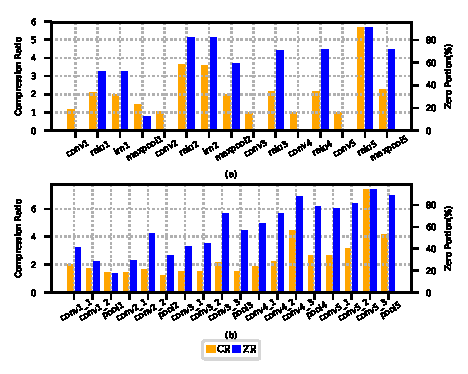
\includegraphics[width=\linewidth]{alexnet_vgg_compression}
\caption{Compression Ratio (CR) and ratio of zero valued neurons (ZR) for different layers of (a) AlexNet and (b) VGG16.}
\label{fig:picCR_VGG}
\end{figure}


